\chapter{Processes}
\begin{tabular}{p{7cm} p{7cm}}
\textbf{processes}			&\textbf{threads}\\
-execution of program			&-several threads share CPU\\
-processor creates virtual processor	&-thread context has little memory information, perhaps mutex lock\\
-for each program everyting is stored in process table	&-threads avoid blocking application (e.g. spreadsheet,computation of dependent cells, intermediate backup)\\
-transparent sharing of resources,(processor, memory) separation&-thread switch is fast\\
-each virtual processor has it's own independent adress space&-user level threads allow parallel computation of program sections\\
-process switch is expensive, (save cpu context, pointers, translation lookaside buffer (TLB), memory management unit (MMU))&I/O or other blocking system calls block all threads, but thread creation/deletion is kernel task = expensive \\
-perhaps even swaps to disk, if memory exhausted& advantages of threads over processes vanishes\\
\end{tabular}

2 possible solutions:\\
\begin{compactenum}
\item scheduler activation, upcall to achieve process switch
\item light-weight processes (LWP)\\
\begin{figure}[h]
	\centering
	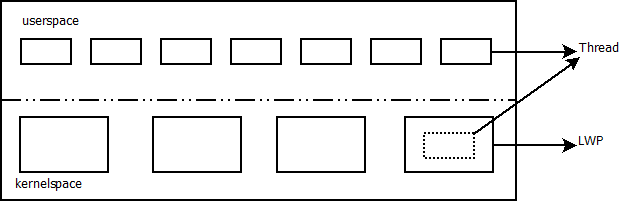
\includegraphics[width=200px]{gfx/thread_lwp.png}
	\caption{light-weight processes can run threads}
	\label{img:lwp_threads}
\end{figure}
user level thread package\\
execute scheduler and run thread of parent\\
may block on systemcall, then other LWP may run\\
triggered from userspace\\
\end{compactenum}
Advantages of LWP and user-level thread package:\\
\begin{compactenum}
\item creation, deletion etc is easy, no kernel intervention
\item blocking syscall does not suspend process if enough LWPs are available
\item applications do not see LWP. They only see user-level threads
\item LWP can run on different processors in multiprocessor systems
\end{compactenum}

Disadvantages:\\
\begin{compactenum}
\item LWP creation as expensive as creation of kernel-level thread
\end{compactenum}

Advantages:\\
- a blocking systemcall blocks only thread, not process
$\Rightarrow$ system call for communication in distributed systems

Multiple threads in clients and servers\\

\textbf{Clients:}\\
\begin{compactitem}
\item multiple thread may hide communication delay (distribution transparency)
\item web browser opens several connections to load parts of a document/page
\item web server may be replicated in same or different location\\
$\Rightarrow$ truly parallel access to items and parallel download
\end{compactitem}

\textbf{Servers:}\\
\begin{compactitem}
\item single threaded, e.g. file server\\
thread serves incoming request, waits for disk, returns file\\
serves next
\item multithreaded\\
dispatcher thread recieves request\\
hands over to worker thread\\
waits for disk etc.\\
dispatcher takes next request
\item finite state machine\\
only one thread\\
examines request, either read from \ldots or from disk\\
during wait stores requests in table\\
serves next request\\
manage control either new request or reply from disk\\
act accordingly\\
process acts as finite state machine that receives messages and acts/changes state
\end{compactitem}

\textbf{summary:}\\
\begin{tabular}{l l}
model&characteristics\\
single thread& no parallelism, blocking syscalls\\
multi thread& parallelism, blocking syscalls\\
finite state machine& parallelism, non-blocking syscalls\\
\end{tabular}

\section{Virtualisation}
% Bild von Höpster
\begin{figure}[h]
	\centering
	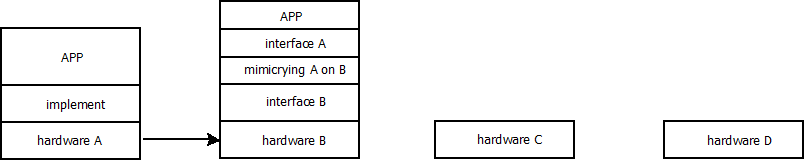
\includegraphics[width=200px]{gfx/virtualisation_1.png}
	\caption{virtualisation}
	\label{img:virtualisation_1}
\end{figure}

V pretends there are more resources then available.\\

Reasons for the need for V.\\
-hardware changes much faster then SW\\
$\Rightarrow$ improves portability\\
-networks consist of different hardware\\
$\Rightarrow$ enables portability of programs for all\\
usage (distributed applications, network protocols)\\

2 Types of Architectures for Virtualisation:\\
\begin{compactenum}
\item Runtime system providing instruction set\\
	\begin{compactitem}
	\item interpreted as Java
	\item emulated as for Windows applications on UNIX-platform processes VM
	\end{compactitem}
\item Virtualisation shields hardware and offers instruction set of the same or other hardware\\
- can host different OS that run simultaneosly\\
$\Rightarrow$ VMM such as VMware, Xen\\


\end{compactenum}


\section{Client-/Serverprocesses}
\textbf{CLients:}\\
%Bild von Tobi !!! :D
\begin{figure}[h]
	\centering
	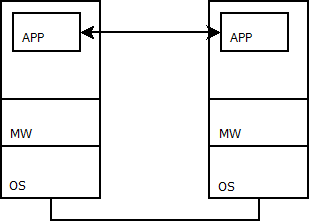
\includegraphics[width=200px]{gfx/clienta.png}
	\caption{app specific communication}
	\label{img:clienta}
\end{figure}
%Mehr Bild!
\begin{figure}[h]
	\centering
	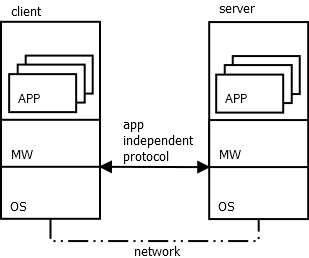
\includegraphics[width=200px]{gfx/clientb.png}
	\caption{machine only communication}
	\label{img:clientb}
\end{figure}

\begin{compactitem}
\item b) allows to store data at the server
\item \textbf{thin client} e.g. X-windows
\item thin client should separate application logic from user interaction
\item ooften not implemented $\Rightarrow$ poor performance
\item compression of interaction commands as solution
\item compound documents where user interaction triggers several processing steps on the server. must be implemented (e.g. rotation of picture changes placement in texts)
\end{compactitem}

\textbf{Servers:}\\
\begin{compactitem}
	\item serves requests on behalf of the client
	\item Types of servers\\
		\begin{compactitem}
			\item \textbf{iterative Server} handles requests itself
			\item \textbf{concurrent server} passes requests to worker, e.g. multithreaded server
		\end{compactitem}
	\item server listens to port, endpoint to the client; some ports are reserved for special services
\begin{figure}[h]
	\centering
	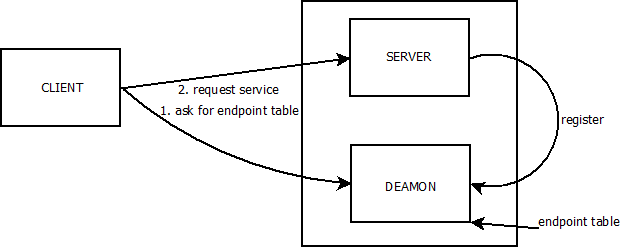
\includegraphics[width=200px]{gfx/server_deamon.png}
	\caption{listener server}
	\label{img:listener}
\end{figure}
	\item superserver listens to several ports, replacinf several (mostly idle) servers
\begin{figure}[h]
	\centering
	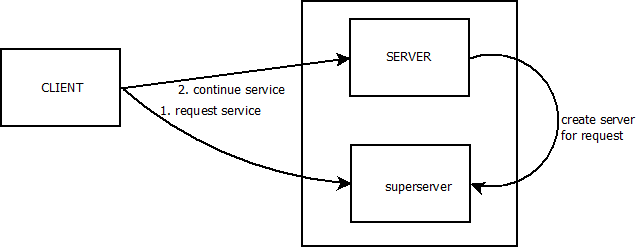
\includegraphics[width=200px]{gfx/superserver.png}
	\caption{superserver}
	\label{img:supserv}
\end{figure}
	\item stateless servers, keeps no information on state of client $\rightarrow$ change state without informing the client, e.g. web server
\begin{figure}[h]
	\centering
	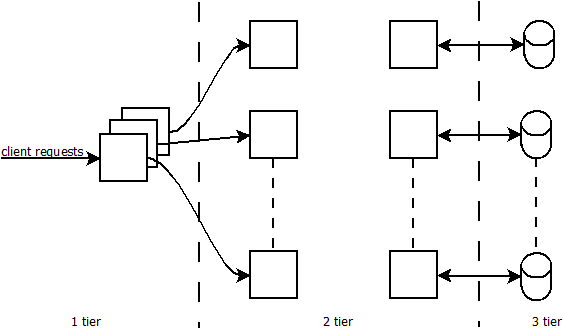
\includegraphics[width=200px]{gfx/server3.png}
	\caption{stateless server}
	\label{img:statel_serv}
\end{figure}
	\item soft state server, maintains client state for limited time, e.g. servers informing about updates
	\item stateful server keeps information about client (file server keeps (client, file) table), often better performance, fault-tolerance poorer
	\item cookies allow to share information for server upon next visit client sends it'S cookies, allows state information for stateless server

\end{compactitem}
\textbf{Distributed Servers}\\
\begin{figure}[h]
	\centering
	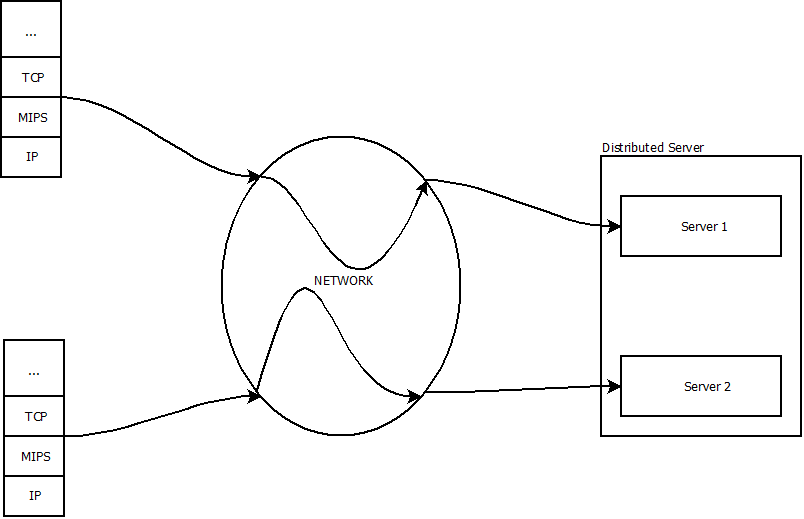
\includegraphics[width=200px]{gfx/distrb_server.png}
	\caption{distributed server}
	\label{img:distrb_serv}
\end{figure}
\begin{compactitem}
	\item servers in different locations that have different ip-adresses in DNS under the same name
	\item MIPv6: mobility support for IPv6
	\item mobile node has home network with stable home adress (HoA)
	\item special router is home agent and takes care of traffic to the mobile node
	\item mobile node receives care-of-adress (CoA), never seen by client
	\item route optimisation avoids routing through home agent
\end{compactitem}

\section{Code Migration}
\begin{compactitem}
	\item Code migration on (running) process - Why?
	\item service placement in distributed system $\Rightarrow$ minimize communication cost
	\item load balancing in multiprocessor machine or cluster $\Rightarrow$ performace
	\item (security)

\end{compactitem}

\textbf{Models of Migration}
\begin{compactitem}
	\item or process model\begin{compactenum}
		\item code segment, instructions
		\item resource segement, references to external resources, ie.e. file, printer, devices
		\item execution segement, execution state process, stack, private data, programm counter

	\end{compactenum}
	\item \textbf{Migration types}\begin{compactitem}
		\item weak mobility, transfer code, (1), mabe 3)), which executes from beginning (i.e. java applets)
		\item strong mobility, transfer 1)3), stop executions, transfer, resume
	\end{compactitem}
\end{compactitem}

%bild

Migrating resource segment 2) is difficult\\
Consider process to resource binding\\
\begin{compactenum}
	\item binding by identifier, URL, ftp-server-name
	\item binding by value, libraries for programming
	\item binding by type, local device, monitor
\end{compactenum}

\textbf{Resource-machine-binding}
\begin{compactenum}
	\item unattached
	\item fastend
	\item fixed
\end{compactenum}

\begin{tabular}{l| l| l| l}
pass tp resource binding&unattached&fastened&fixed\\
\hline
by identifier& MV&GR(or MV)& GR\\
\hline
by value& CP& GR(or CP)& GR\\
\hline
by type& RB&RB(or GR,CP)&RB(or GR)\\
\end{tabular}
MV:move, GR, global reference, CP: copy value, RB: rebind to locally available resource

